\sectionframe{Basic data types and operators}
\begin{frame}
 \frametitle{Structure of a simple assignment command}
 \begin{figure}
  \centering
  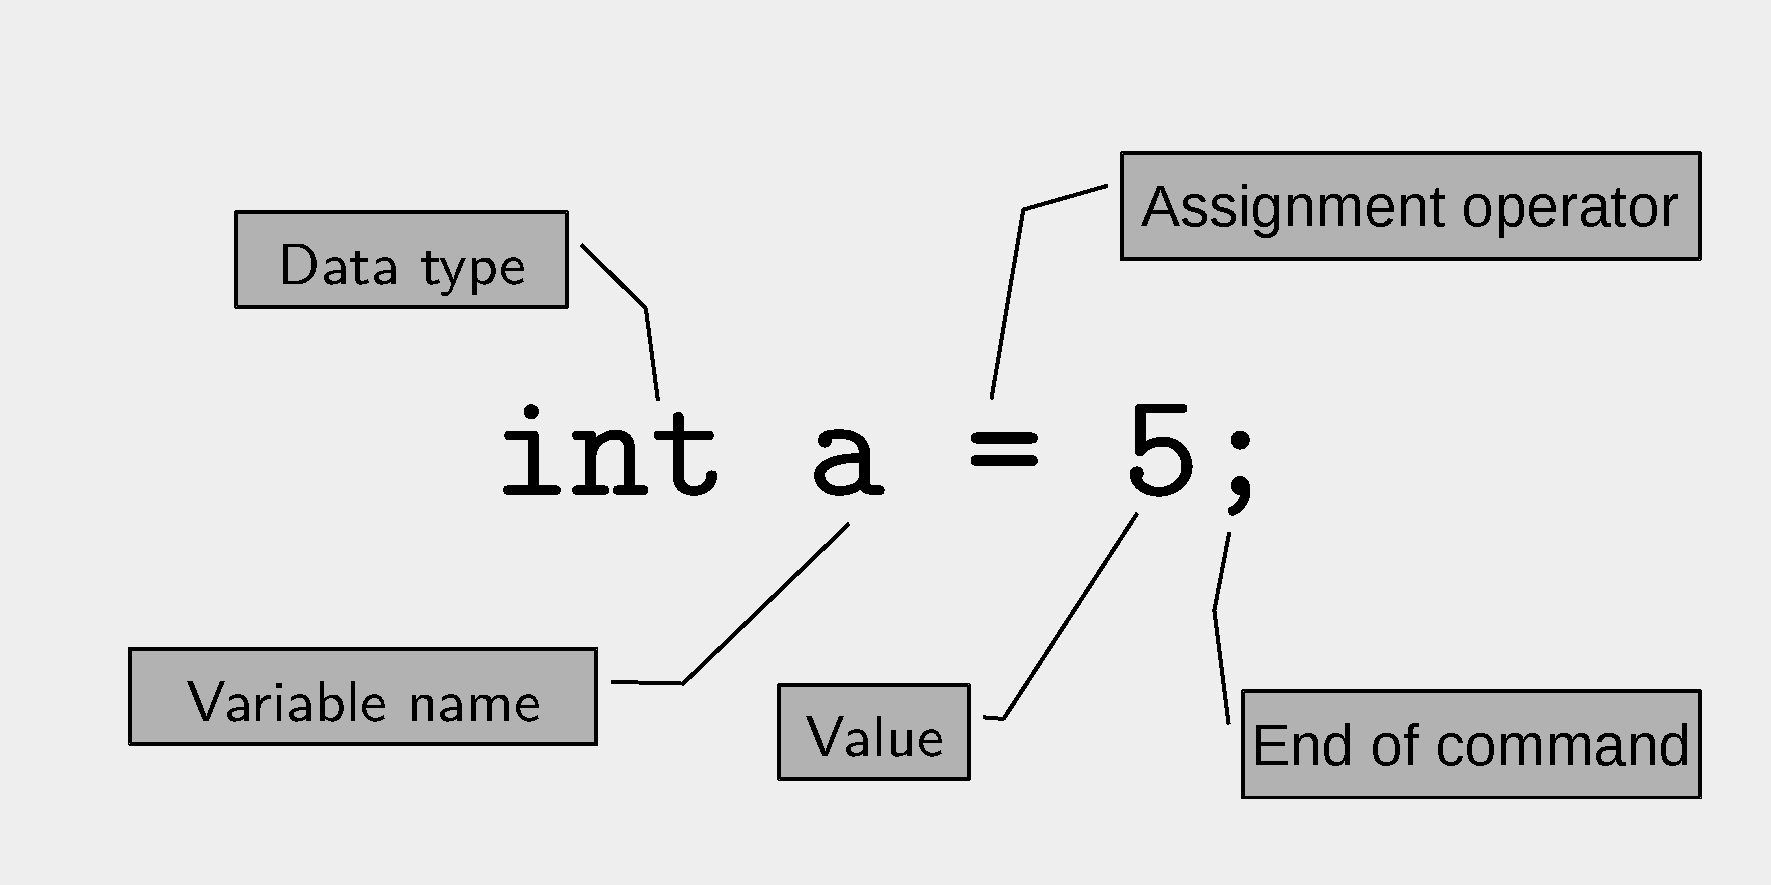
\includegraphics[width=\linewidth]{Bilder/OPL-Anweisung}
 \end{figure}
\end{frame}

\shorthandoff{"}
\subsection{Data types}
\begin{frame}
 \frametitle{Primitive data types}
 \begin{description}
  \item[\texttt{int}] short for: ``integer'', an integer value with arbitrary sign. 
  Example literals: \texttt{\usebeamercolor[fg]{example text}0, 1, -2, -786}
  \item[\texttt{float}] floating point number with arbitrary sign.
  Example literals: \texttt{\usebeamercolor[fg]{example text}0.0, 1.0, 3.14, -7.86}
  \item[\texttt{boolean}] technically a logical value; as decision variable a 0-1-variable.
  \shorthandoff{"}
  \item[\texttt{string}] a charachter string. Example literals:
  \texttt{\usebeamercolor[fg]{example text} "1", "B", "Berlin"}
  \shorthandon{"}
 \end{description}
\end{frame}


\begin{frame}
 \frametitle{Derived data types}
 \begin{description}
  \item[Set] an ordered set of elements of (i.a.) primitve data types, e.g.
  \begin{flushleft}\ttfamily\usebeamercolor[fg]{example text}
  \{string\} Locations =\\\ \{"Ansbach", "Berlin", "Cottbus"\};
  \end{flushleft}
  \item[Array] a tuple of (i.a.) primitive data type, sets and other arrays indexed over a set, e.g.
  \begin{flushleft}\ttfamily\usebeamercolor[fg]{example text}
  float Fixcosts[Locations] =\\\ [27.4, 58.3, 30.0];
  \end{flushleft}
  access by index, z.B.: \texttt{\usebeamercolor[fg]{example text}Fixcosts["Cottbus"]} \textrightarrow{} \texttt{\usebeamercolor[fg]{example text}30.0}
 \end{description}
\end{frame}
\shorthandon{"}

\begin{frame}
 \frametitle{Derived data types: mutiple arrays}
 \begin{itemize}
  \item Arrays can be nested into one another to represent multiple indexes, e.g.
    \begin{flushleft}\ttfamily\usebeamercolor[fg]{example text}
      float Entf[Locations][Locations] =\\ 
      \ [[0.0, 5.05, 4.89],\\
      \ [5.05, 0.0, 1.22],\\
      \ [4.89, 1.22, 0.0]];
    \end{flushleft}
  \item Mapping rule: from left to right, from outer to inner
 \end{itemize}
\end{frame}

\subsection{Operators}
\begin{frame}
 \frametitle{Simple Operators}
 \begin{itemize}
  \item assignment operator \structure{\texttt{=}}
  \item arithmetic operators
  \begin{description}
   \item[\texttt{+}] addition
   \item[\texttt{-}] subtraction
   \item[\texttt{*}] multiplication
   \item[\texttt{/}] division (rare in linear models)
  \end{description}
  \item comparison operator (for linear models)
  \begin{description}
   \item[\texttt{==}] equal
   \item[\texttt{<=}] less or equal
   \item[\texttt{>=}] greater or equal
  \end{description}
 \end{itemize}
\end{frame}

\begin{frame}
 \frametitle{Indexed operators}
 \begin{itemize}
  \item sum operator
  \begin{flushleft}\Large
   {\usebeamercolor[fg]{example text}$\displaystyle\sum_{\alert{i}\in \alert{I}}\ldots$} 
   \textrightarrow{} 
   {\usebeamercolor[fg]{example text} \texttt{sum(\alert{i} in \alert{I})(\textsf{...})}}
  \end{flushleft}
  \medskip
  \item universal quantifier
  \begin{flushleft}\Large
   {\usebeamercolor[fg]{example text}$\displaystyle\forall {\alert{i}\in \alert{I}}$} 
   \textrightarrow{} 
   {\usebeamercolor[fg]{example text} \texttt{forall(\alert{i} in \alert{I})}}
  \end{flushleft}
 \end{itemize}

\end{frame}


